\documentclass[a4paper,11pt]{article}
\usepackage{geometry}
 \geometry{
 a4paper,
 total={170mm,257mm},
 left=20mm,
 top=20mm,
 }

 \usepackage{multirow}
\usepackage{colortbl}
 \usepackage{hhline}

 \usepackage{lipsum}  %%% Lorem ipsum

\setlength{\headheight}{30.0pt}
\setlength{\footskip}{20pt}



\usepackage{hyperref}
\hypersetup{
    colorlinks=True,
    linkcolor={blue!20!black},
    filecolor=magenta,      
    urlcolor=cyan,
}



 \usepackage[export]{adjustbox}
\usepackage[english]{babel}
\usepackage[utf8]{inputenc}
\usepackage{fancyhdr}
\usepackage{multicol}

\pagestyle{fancy}
\fancyhf{}
\rhead{\textit{Pul074BEX004}}
\lhead{\textit{Amrit Prasad Phuyal}}
\rfoot{\thepage}


\usepackage{mathpazo} % Palatino font
\usepackage{graphicx}
\usepackage{float}

%%%% Anser environment use %%%% Anser environment use %%%% Anser environment use \input{./AnsENV.tex}
%% use \begin{A... {**** argument***}
\RequirePackage{scrextend}

\newenvironment{A}[1]{\textit{Answer:}{\begin{addmargin}[2em]{2em}{#1}\end{addmargin} 
  }}

% just leave some space   
%% use \begin{A... {**** argument***}
\RequirePackage{scrextend}

\newenvironment{A}[1]{\textit{Answer:}{\begin{addmargin}[2em]{2em}{#1}\end{addmargin} 
  }}

% just leave some space   
%% use \begin{A... {**** argument***}
\RequirePackage{scrextend}

\newenvironment{A}[1]{\textit{Answer:}{\begin{addmargin}[2em]{2em}{#1}\end{addmargin} 
  }}

% just leave some space    %% Answer environment 

%%% Question Environment%%%  use 
%%% Question Environment%%%  use 
%%% Question Environment%%%  use \input{./QueENV.tex}   to include
%% Use \begin{Q}....\end{Q}

\newcounter{QC}
\setcounter{QC}{1}
\newenvironment{Q}[1]{
    \section{Question -\arabic{QC}} \stepcounter{QC}{\large\textbf{#1}}
}

%%% Question Environment%%%

   to include
%% Use \begin{Q}....\end{Q}

\newcounter{QC}
\setcounter{QC}{1}
\newenvironment{Q}[1]{
    \section{Question -\arabic{QC}} \stepcounter{QC}{\large\textbf{#1}}
}

%%% Question Environment%%%

   to include
%% Use \begin{Q}....\end{Q}

\newcounter{QC}
\setcounter{QC}{1}
\newenvironment{Q}[1]{
    \section{Question -\arabic{QC}} \stepcounter{QC}{\large\textbf{#1}}
}

%%% Question Environment%%%

 %% Question Environment 
%%%%%% include  Titles.%%%% use \input{./CP}%%%
%%%use """"""""    \CP{}{}{}{}   """" %%%% and 4 argument to craete Title page 
%%%%%%%%%%%%%%%%%%%%%%%%%%%%%%%%%%%%%%%%%%%%%%%%%%%%%%%%%%%%%%%%%
%%%argument number
%% 1=major header ## Course name 
%% 2=minor4 heading ## lab/assignmet no
%% 3=Title  ## Assignment or Lab title
%% 4=submitted to::## input receiver Name"
%%%%%%%%%%%%%%%%%%%%%%%%%%%%%%%%%%%%%%%%%%%%%%%%%%%%%%%%%%%%%%%%%


\usepackage{mathpazo} % Palatino font
\usepackage{graphicx}
\usepackage{float}

%%% format and command for lab ans c and assembly

\newcommand{\HRule}{\rule{\linewidth}{0.4mm}} % Defines a new command for horizontal lines, change thickness here



%----------------------------------------------------------------------------------------
%	TITLE PAGE
%----------------------------------------------------------------------------------------


\newcommand{\CP}[4]{ \begin{titlepage} % Suppresses displaying the page number on the title page and the subsequent page counts as page 1
		%%%%  univerdity logo%%
		\begin{figure}[H]
			\centering
			
\includegraphics[scale=0.13]{tulogo.jpg}
		\end{figure}
		%%% end university logo

		\center % Centre everything on the page

		%------------------------------------------------
		%	Headings
		%------------------------------------------------

		\textsc{\huge Institute of Engineering \\ Central Campus,Pulchowk}\\[1.5cm] % Main heading such as the name of your university/college

		\textsc{\Large #1}\\[0.5cm] % Major heading such as course name

		\textsc{\large #2}\\[0.5cm] % Minor heading such as assignment no./ lab no.

		%------------------------------------------------
		%	Title
		%------------------------------------------------

		\HRule\\[0.4cm]

		{\Huge\bfseries #3}\\[0.4cm] % Title of your document

		\HRule\\[1.5cm]

		%------------------------------------------------
		%	Author(s)
		%------------------------------------------------
		\vfill\vfill
		\begin{minipage}{0.4\textwidth}
			\begin{flushleft}
				\large{
				\textbf{Submitted BY:}\\
				{\normalsize AMRIT PRASAD PHUYAL}\\ % NAME
				{\normalsize Roll: PULL074BEX004}} % Roll
			\end{flushleft}
		\end{minipage}
		~
		\begin{minipage}{0.4\textwidth}
			\begin{flushright}
				\large
				\textbf{Submitted To:}\\
				{ \normalsize{#4}\\ }% recepent's  Name 
				{\normalsize Department of Electronics and Computer Engineering}
			\end{flushright}
		\end{minipage}

		%------------------------------------------------
		%	Date
		%------------------------------------------------

		\vfill\vfill\vfill % Position the date 3/4 down the remaining page

		{\large\today} % Date, change the \today to a set date if you want to be precise

		\vfill % Push the date up 1/4 of the remaining page

	\end{titlepage}
} %%% cover page

%%% For CMD output %%%

%%%%%%%%% use  
%%% For CMD output %%%

%%%%%%%%% use  
%%% For CMD output %%%

%%%%%%%%% use  \include{CMD output.tex}
%%%%%%%%% use \CMD{###filename}{##Caption}
\usepackage{listings}

\usepackage{mdframed}
\usepackage{xcolor}
%\definecolor{codegreen}{rgb}{0,0.6,0}
%\definecolor{codegray}{rgb}{0.4,0.4,0.4}
%\definecolor{codepurple}{rgb}{0.58,0,0.82}
%\definecolor{blackcolour}{rgb}{0,0,0}


\definecolor{bluefront}{RGB}{10,214,255}
\definecolor{blueback}{RGB}{25,24,96}


\renewcommand{\lstlistlistingname}{List of CMD Outputs}
\renewcommand{\lstlistingname}{Output}


\lstdefinestyle{customa}{
    backgroundcolor=\color{blueback},
    %  keywordstyle=\color{magenta},
    %numberstyle=\tiny\color{codegray},
    %stringstyle=\color{codepurple},
    basicstyle=\ttfamily\scriptsize\color{bluefront},
    breakatwhitespace=false,
    breaklines=true,
    captionpos=b,
    %morekeywords={MOV,ADD,ADDC,ACALL,INC,DJNZ,AJMP,RET,END,ORG,RR,JNC,SUBB,JC,DEC},
    keepspaces=true,
    %numbers=left,
    %numbersep=5pt,
    showspaces=false,
    showstringspaces=false,
    showtabs=false,
    tabsize=4
}

\newcommand {\CMD}[2]{

    \begin{mdframed}[backgroundcolor=blueback,innerbottommargin=-2.3em,innertopmargin=-0.1em]
        \lstinputlisting[style=customa,caption={#2}]{#1}
    \end{mdframed}
}

%%% For CMD output %%%


%%%%%%%%% use \CMD{###filename}{##Caption}
\usepackage{listings}

\usepackage{mdframed}
\usepackage{xcolor}
%\definecolor{codegreen}{rgb}{0,0.6,0}
%\definecolor{codegray}{rgb}{0.4,0.4,0.4}
%\definecolor{codepurple}{rgb}{0.58,0,0.82}
%\definecolor{blackcolour}{rgb}{0,0,0}


\definecolor{bluefront}{RGB}{10,214,255}
\definecolor{blueback}{RGB}{25,24,96}


\renewcommand{\lstlistlistingname}{List of CMD Outputs}
\renewcommand{\lstlistingname}{Output}


\lstdefinestyle{customa}{
    backgroundcolor=\color{blueback},
    %  keywordstyle=\color{magenta},
    %numberstyle=\tiny\color{codegray},
    %stringstyle=\color{codepurple},
    basicstyle=\ttfamily\scriptsize\color{bluefront},
    breakatwhitespace=false,
    breaklines=true,
    captionpos=b,
    %morekeywords={MOV,ADD,ADDC,ACALL,INC,DJNZ,AJMP,RET,END,ORG,RR,JNC,SUBB,JC,DEC},
    keepspaces=true,
    %numbers=left,
    %numbersep=5pt,
    showspaces=false,
    showstringspaces=false,
    showtabs=false,
    tabsize=4
}

\newcommand {\CMD}[2]{

    \begin{mdframed}[backgroundcolor=blueback,innerbottommargin=-2.3em,innertopmargin=-0.1em]
        \lstinputlisting[style=customa,caption={#2}]{#1}
    \end{mdframed}
}

%%% For CMD output %%%


%%%%%%%%% use \CMD{###filename}{##Caption}
\usepackage{listings}

\usepackage{mdframed}
\usepackage{xcolor}
%\definecolor{codegreen}{rgb}{0,0.6,0}
%\definecolor{codegray}{rgb}{0.4,0.4,0.4}
%\definecolor{codepurple}{rgb}{0.58,0,0.82}
%\definecolor{blackcolour}{rgb}{0,0,0}


\definecolor{bluefront}{RGB}{10,214,255}
\definecolor{blueback}{RGB}{25,24,96}


\renewcommand{\lstlistlistingname}{List of CMD Outputs}
\renewcommand{\lstlistingname}{Output}


\lstdefinestyle{customa}{
    backgroundcolor=\color{blueback},
    %  keywordstyle=\color{magenta},
    %numberstyle=\tiny\color{codegray},
    %stringstyle=\color{codepurple},
    basicstyle=\ttfamily\scriptsize\color{bluefront},
    breakatwhitespace=false,
    breaklines=true,
    captionpos=b,
    %morekeywords={MOV,ADD,ADDC,ACALL,INC,DJNZ,AJMP,RET,END,ORG,RR,JNC,SUBB,JC,DEC},
    keepspaces=true,
    %numbers=left,
    %numbersep=5pt,
    showspaces=false,
    showstringspaces=false,
    showtabs=false,
    tabsize=4
}

\newcommand {\CMD}[2]{

    \begin{mdframed}[backgroundcolor=blueback,innerbottommargin=-2.3em,innertopmargin=-0.1em]
        \lstinputlisting[style=customa,caption={#2}]{#1}
    \end{mdframed}
}

%%% For CMD output %%%

 %%% Cmd OUTPUT blue background


\begin{document}


%%%%  COver page 
\CP{Computer Network}{Lab \#6}{To Introduce the Concept of Subnetting, Subnet Mask, VLSM and CIDR}
{SHARAD KUMAR GHIMIRE}
%%%%%%%%%%%%%%%%%%%%

\pagenumbering{gobble}
\renewcommand{\contentsname}{Table of Contents}
\tableofcontents

%\pagebreak
%\listoffigures
% \pagebreak
% \listoftables
\pagebreak
\lstlistoflistings
\pagebreak
\listoffigures
\pagebreak
\pagenumbering{arabic}

\section{Title} {\large To Introduce the Concept of Subnetting, Subnet Mask, VLSM and CIDR}
%%%%%%%%%%%%%%%%%%%%%%%%%%%%
\section{Objective}
\begin{itemize}
    \item To be familiar with subnetting, subnet mask and its use
    \item To be familiar with VLSM and CIDR

\end{itemize}
%%%%%%%%%%%%%%%%%%%%%
\section{Requirement}
\begin{itemize}
    \item Network simulation tool: Packet Tracer
\end{itemize}
%%%%%%%%%%%%%%%%%%%

\section{Procedure}

With the help of Cisco Packet Tracer we simulated Subnetting of  different IP ranges also explored  VLSM (Variable Length Subnet Mask) and  CIDR (Classless Inter-Domain Routing).
We performed Ping Operation to visualize the concept of Subnet and prove that to communicate between different network Router is required.



\pagebreak
%%%%%%%%%%%%%%%%%%%%%%%%%%%%%%%%%%%%%%%%%%%%%%%%%%%%%%%%%%%%%%%%%%%%%%%%%%%%%%%%%%%%%%%%%%%%%%%%
\section{Exercises:}
%%%%%%%%%%%%%%%%%%%%%%%%%11111111111111111111111

\begin{Q}
    {
        Observe and note down the output of each of the above mentioned task and comment on
        the result by explaining the reason in detail.
    }
\end{Q}

%
%
%
%

%%%%%%%%%%%%%%%%%%%%%%AAAAAAAAAAAAAAAAAAAAAAAAAAAAAAAA
%%%%%%%%%%%%%%%%%%%%%%AAAAAAAAAAAAAAAAAAAAAAAAAAAAAAAA
%%%%%%%%%%%%%%%%%%%%%%AAAAAAAAAAAAAAAAAAAAAAAAAAAAAAAA
%%%%%%%%%%%%%%%%%%%%%%AAAAAAAAAAAAAAAAAAAAAAAAAAAAAAAA
%%%%%%%%%%%%%%%%%%%%%%AAAAAAAAAAAAAAAAAAAAAAAAAAAAAAAA

%
%
%

\addtocontents{lol}{\protect\subsection*{\HRule \\ Activities A\\ \HRule}}

\addtocontents{lof}{\protect\subsection*{\HRule \\ Activities A\\ \HRule}}

\subsubsection{Activities A}

{\bfseries \textit{A. Create the network topology as shown in figure 1 below, and note down the output by performing the following activities:}}

\begin{figure}[H]
    \centering
    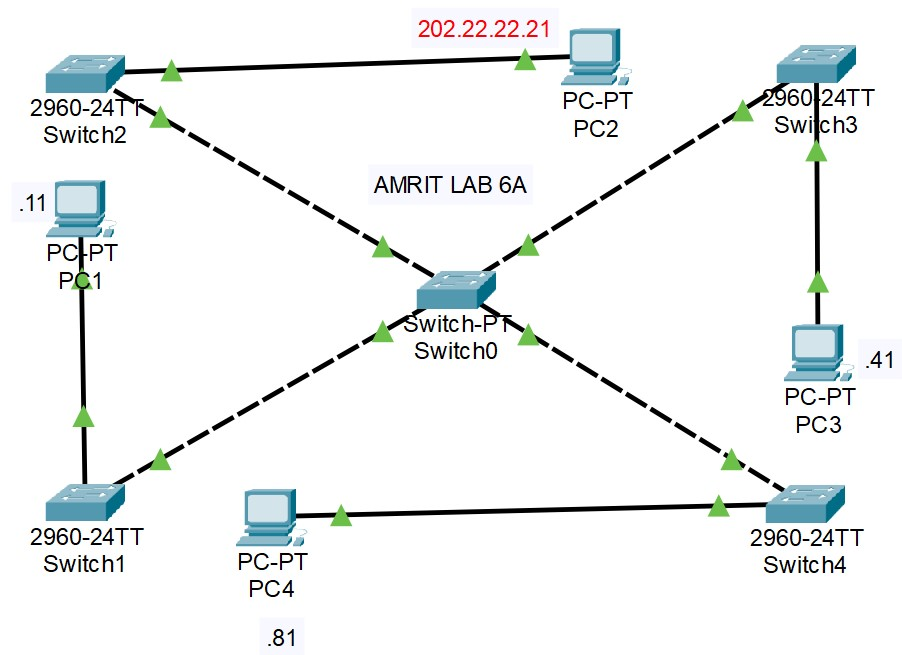
\includegraphics[scale=0.9,cframe=blue 0.5pt 3pt]{./FIG/Lab6A.jpg}
    \caption{Network topology Lab 6A}
\end{figure}


\begin{enumerate}
    \item \textbf{ Assign the IP address of PC1, PC2, PC3 and PC4 as 202.22.22.11, 202.22.22.21,
              202.22.22.41, 202.22.22.81 respectively with subnet mask of 255.255.255.0 and note down
              the result of following operations:}
          \begin{figure}[H]
              \centering
              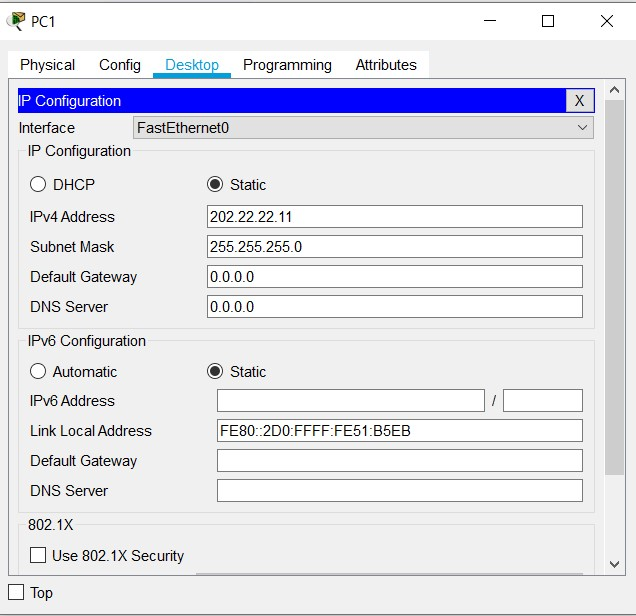
\includegraphics[scale=0.8,cframe=blue 0.5pt 3pt]{./FIG/APC1.jpg}
              \caption{Assign IP address and subnet mask for PC1}
          \end{figure}



    \item \textbf{ Test the connectivity from one computer to all another computers using ping.}

          \addtocontents{lol}{\protect\subsubsection*{A.2: Subnet mask : 255.255.255.0}}

          \CMD{./CODES/A2P1-4.txt}{Ping from PC1 to PC4}
          \CMD{./CODES/A2P2-1.txt}{Ping from PC2 to PC1}
          \CMD{./CODES/A2P3-2.txt}{Ping from PC3 to PC2}
          \CMD{./CODES/A2P4-3.txt}{Ping from PC4 to PC3}

          Since subnet mask is (/24) it covers usable host from 202.22.22.0 - 202.22.22.254 in a single network so ping is possible between and among the PCs with the help of switching device only.


    \item \textbf{ Change the subnet mask to 255.255.255.192 and test the connectivity from one computer
              to all another computers using ping.}

          \addtocontents{lol}{\protect\subsubsection*{A.3: Subnet mask : 255.255.255.192}}

          \CMD{./CODES/A3P1-4.txt}{Ping from PC1 to PC4}
          \CMD{./CODES/A3P2-1.txt}{Ping from PC2 to PC1}
          \CMD{./CODES/A3P3-2.txt}{Ping from PC3 to PC2}
          \CMD{./CODES/A3P4-3.txt}{Ping from PC4 to PC3}

          \begin{figure}[H]
              \centering
              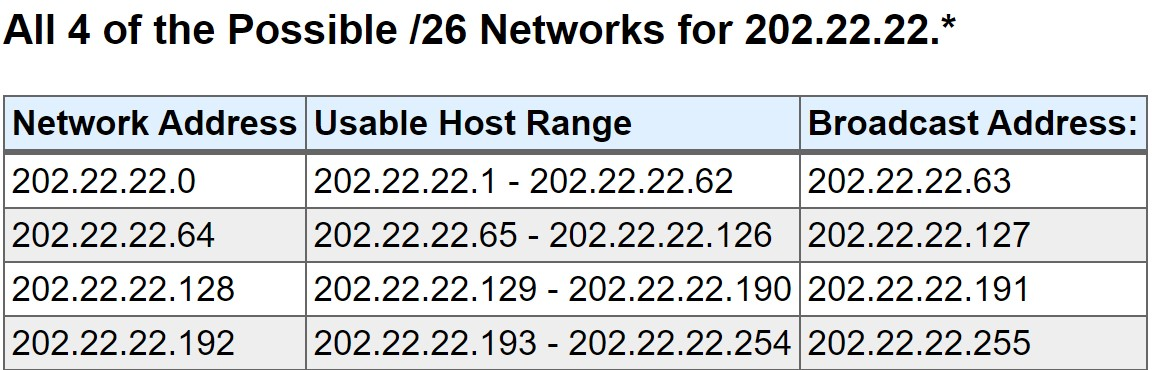
\includegraphics[scale=0.7,cframe=blue 0.5pt 3pt]{./FIG/A26.jpg}
              \caption{Possible subnets for /26 }
          \end{figure}


          With subnet mask (/26)  PC1, PC1 and PC3 falls under same subnet  and PC4 under different subnet so ping failed to and from PC4 but successful among PC1, PC2, PC3.


    \item \textbf{ Change the subnet mask to 255.255.255.224 and test the connectivity from one computer
              to all another computers using ping.}

          \addtocontents{lol}{\protect\subsubsection*{A.3: Subnet mask : 255.255.255.224}}

          \CMD{./CODES/A4P1-4.txt}{Ping from PC1 to PC4}
          \CMD{./CODES/A4P2-1.txt}{Ping from PC2 to PC1}
          \CMD{./CODES/A4P3-2.txt}{Ping from PC3 to PC2}
          \CMD{./CODES/A4P4-3.txt}{Ping from PC4 to PC3}

          \begin{figure}[H]
              \centering
              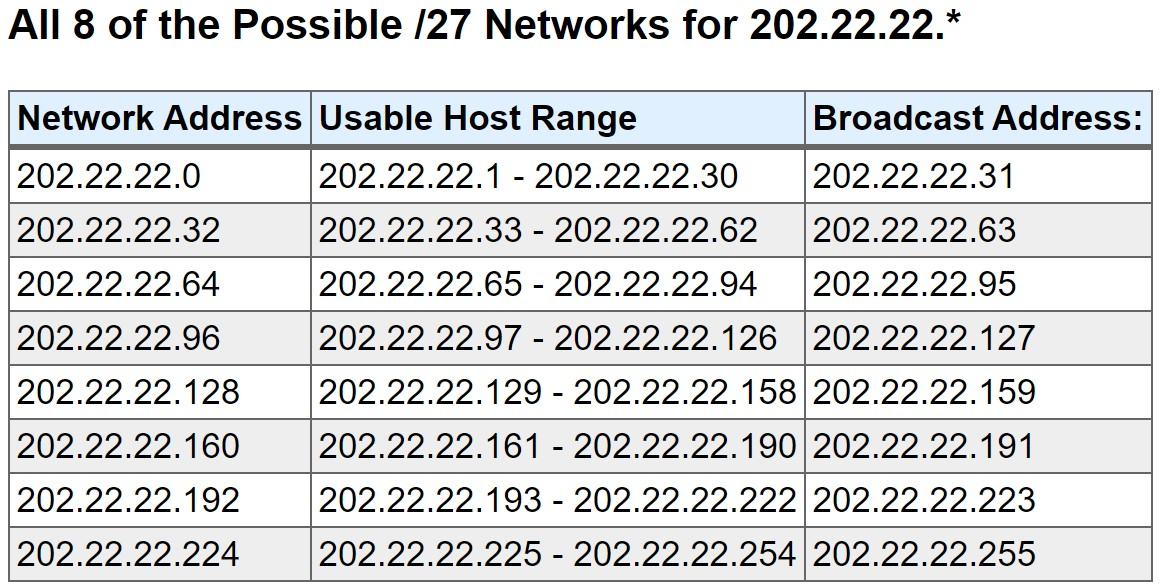
\includegraphics[scale=0.7,cframe=blue 0.5pt 3pt]{./FIG/A27.jpg}
              \caption{Possible subnets for /27 }
          \end{figure}

          With subnet (/27) only PC1 and PC2 falls under a same subnet and ping is possible between them  but as PC3 and PC4 falls under different subnet ping failed to and from (PC1, PC2) , PC3 and  PC4.


    \item \textbf{ Change the subnet mask to 255.255.255.240 and test the connectivity from one computer
              to all another computers using ping.}


          \addtocontents{lol}{\protect\subsubsection*{A.3: Subnet mask : 255.255.255.240}}

          \CMD{./CODES/A5P1-4.txt}{Ping from PC1 to PC4}
          \CMD{./CODES/A5P2-1.txt}{Ping from PC2 to PC1}
          \CMD{./CODES/A5P3-2.txt}{Ping from PC3 to PC2}
          \CMD{./CODES/A5P4-3.txt}{Ping from PC4 to PC3}

          \begin{figure}[H]
              \centering
              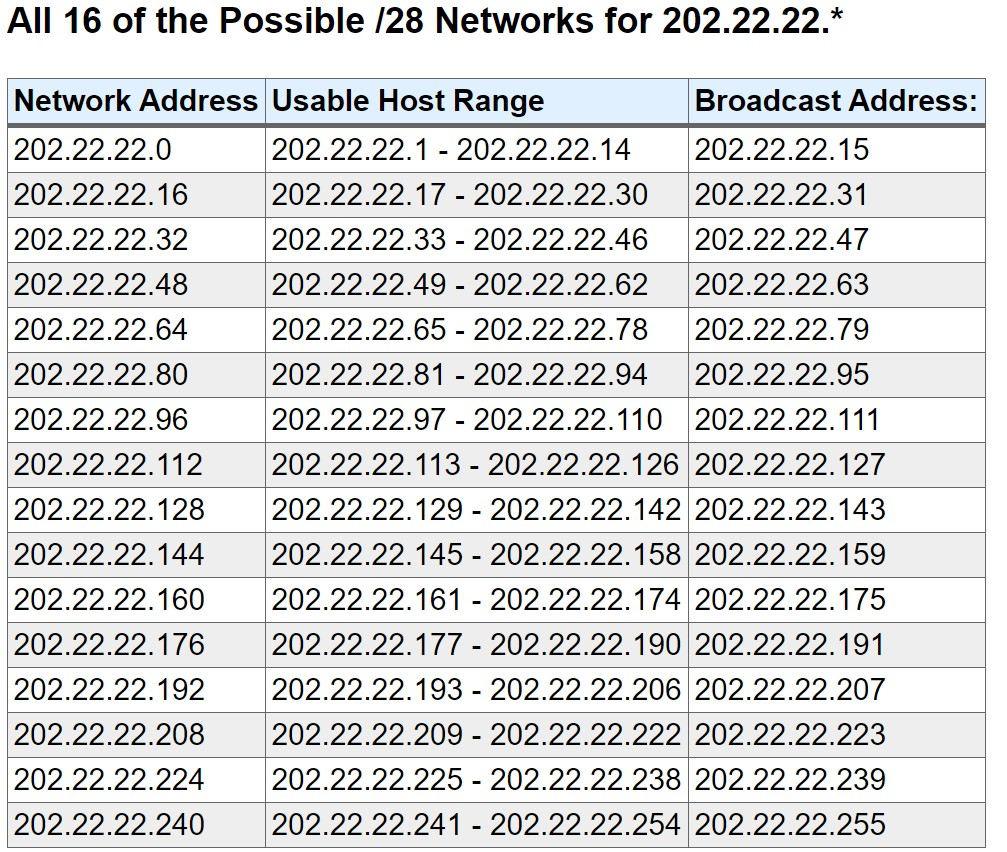
\includegraphics[scale=0.8,cframe=blue 0.5pt 3pt]{./FIG/A28.jpg}
              \caption{Possible subnets for /28 }
          \end{figure}

          With subnet mask  (/28) all PCs falls under different subnet and Ping Failed between each PCs.

\end{enumerate}

\pagebreak
%
%
%
%
%%%%%%%%%%%%%%%%%%%%%%%%%%%BBBBBBBBBBBBBBBBBBBBB
%%%%%%%%%%%%%%%%%%%%%%%%%%%BBBBBBBBBBBBBBBBBBBBB
%%%%%%%%%%%%%%%%%%%%%%%%%%%BBBBBBBBBBBBBBBBBBBBB
%%%%%%%%%%%%%%%%%%%%%%%%%%%BBBBBBBBBBBBBBBBBBBBB
%%%%%%%%%%%%%%%%%%%%%%%%%%%BBBBBBBBBBBBBBBBBBBBB
%
%
%
%
\addtocontents{lol}{\protect\subsection*{\HRule \\ Activities B\\ \HRule}}

\addtocontents{lof}{\protect\subsection*{\HRule \\ Activities B\\ \HRule}}

\subsubsection{Activities B}

{\bfseries \textit{B. For the situation given in 5 of activity A above, replace the central switch i.e. switch0 by a router and configure its interfaces with appropriate IP address and subnet mask. Also configure each computer with default gateway. Test the connectivity from one computer to all another computers using ping.}}


\begin{figure}[H]
    \centering
    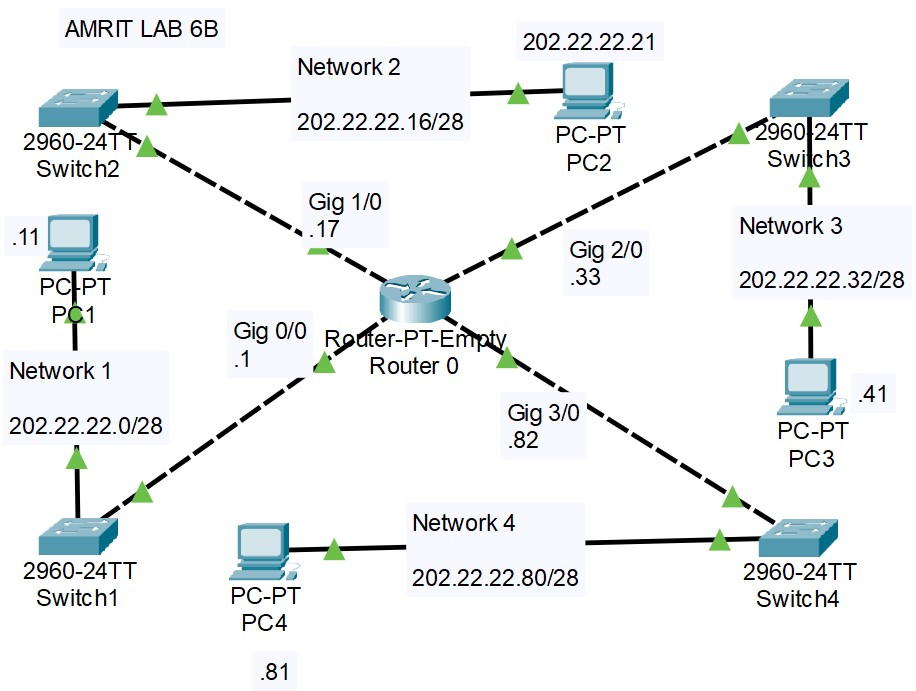
\includegraphics[scale=0.9,cframe=blue 0.5pt 3pt]{./FIG/Lab6B.jpg}
    \caption{Network topology Lab 6B}
\end{figure}

\addtocontents{lol}{\protect\subsubsection*{Router at center with Subnet mask : 255.255.255.240}}

\CMD{./CODES/BP1-4.txt}{Ping from PC1 to PC4}
\CMD{./CODES/BP2-1.txt}{Ping from PC2 to PC1}
\CMD{./CODES/BP3-2.txt}{Ping from PC3 to PC2}
\CMD{./CODES/BP4-3.txt}{Ping from PC4 to PC3}


In the Activity A.5 we illustrate that all PCs falls under different subnet and as we know Router is needed to communicate between different network. Here in this activity we used Router  between the PCs of different Network  which makes the Ping Successful from any PCS to any other PCs.






\pagebreak

%
%
%
%
%
%%%%%%%%%%%%%%%%%%%%%%%%%CCCCCCCCCCCCCCCCCCCCCCCCCCCC
%%%%%%%%%%%%%%%%%%%%%%%%%CCCCCCCCCCCCCCCCCCCCCCCCCCCC
%%%%%%%%%%%%%%%%%%%%%%%%%CCCCCCCCCCCCCCCCCCCCCCCCCCCC
%%%%%%%%%%%%%%%%%%%%%%%%%CCCCCCCCCCCCCCCCCCCCCCCCCCCC
%%%%%%%%%%%%%%%%%%%%%%%%%CCCCCCCCCCCCCCCCCCCCCCCCCCCC
%
%
%
%

\addtocontents{lol}{\protect\subsection*{\HRule \\ Activities C\\ \HRule}}

\addtocontents{lof}{\protect\subsection*{\HRule \\ Activities C\\ \HRule}}

\subsubsection{Activities C}

{\bfseries \textit{C. Create the network topology as shown in figure 1 above and Assign the IP address of PC1,  PC2, PC3 and PC4 as 202.44.8.2, 202.44.9.2, 202.44.10.2 and 202.44.11.2 respectively with subnet mask of 255.255.255.0 and note down the result of following operations}}


\begin{figure}[H]
    \centering
    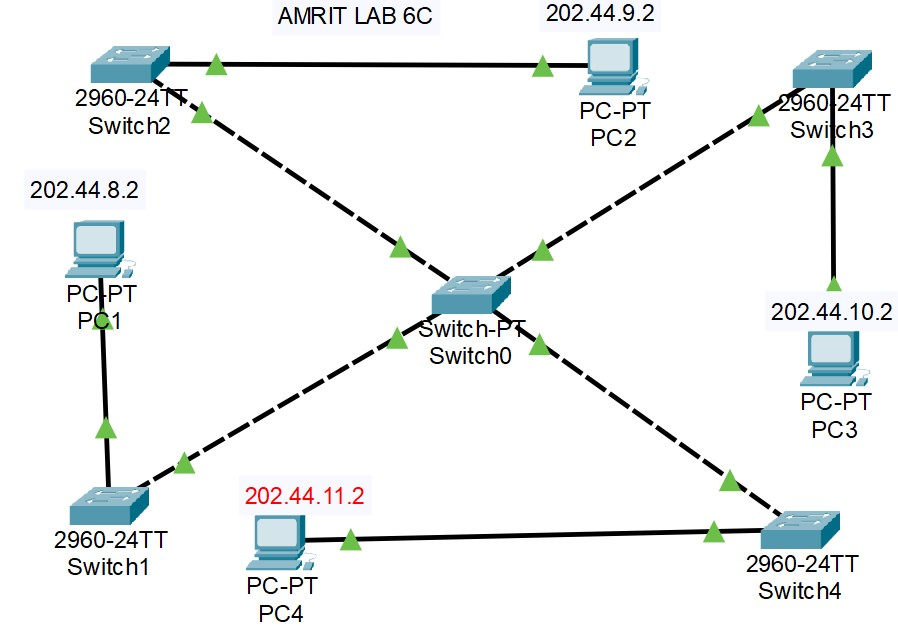
\includegraphics[scale=0.9,cframe=blue 0.5pt 3pt]{./FIG/Lab6C.jpg}
    \caption{Network topology Lab 6C}
\end{figure}



\begin{enumerate}
    \item \textbf{ Test the connectivity from one computer to another using ping.}


          \addtocontents{lol}{\protect\subsubsection*{C.2: Subnet mask : 255.255.255.0}}

          \CMD{./CODES/C2P1-4.txt}{Ping from PC1 to PC4}
          \CMD{./CODES/C2P2-1.txt}{Ping from PC2 to PC1}
          \CMD{./CODES/C2P3-2.txt}{Ping from PC3 to PC2}
          \CMD{./CODES/C2P4-3.txt}{Ping from PC4 to PC3}


          With subnet mask (/24) all PCs falls under different subnet  and with the help of Switch communication between the PCs of different subnet is impossible so Ping Failed between all PCs.



    \item \textbf{ Change the subnet mask to 255.255.254.0 and test the connectivity from one computer to
              another using ping.}

          \addtocontents{lol}{\protect\subsubsection*{C.3: Subnet mask : 255.255.254.0}}

          \CMD{./CODES/C3P1-4.txt}{Ping from PC1 to PC4}
          \CMD{./CODES/C3P2-1.txt}{Ping from PC2 to PC1}
          \CMD{./CODES/C3P3-2.txt}{Ping from PC3 to PC2}
          \CMD{./CODES/C3P4-3.txt}{Ping from PC4 to PC3}

          \begin{figure}[H]
              \centering
              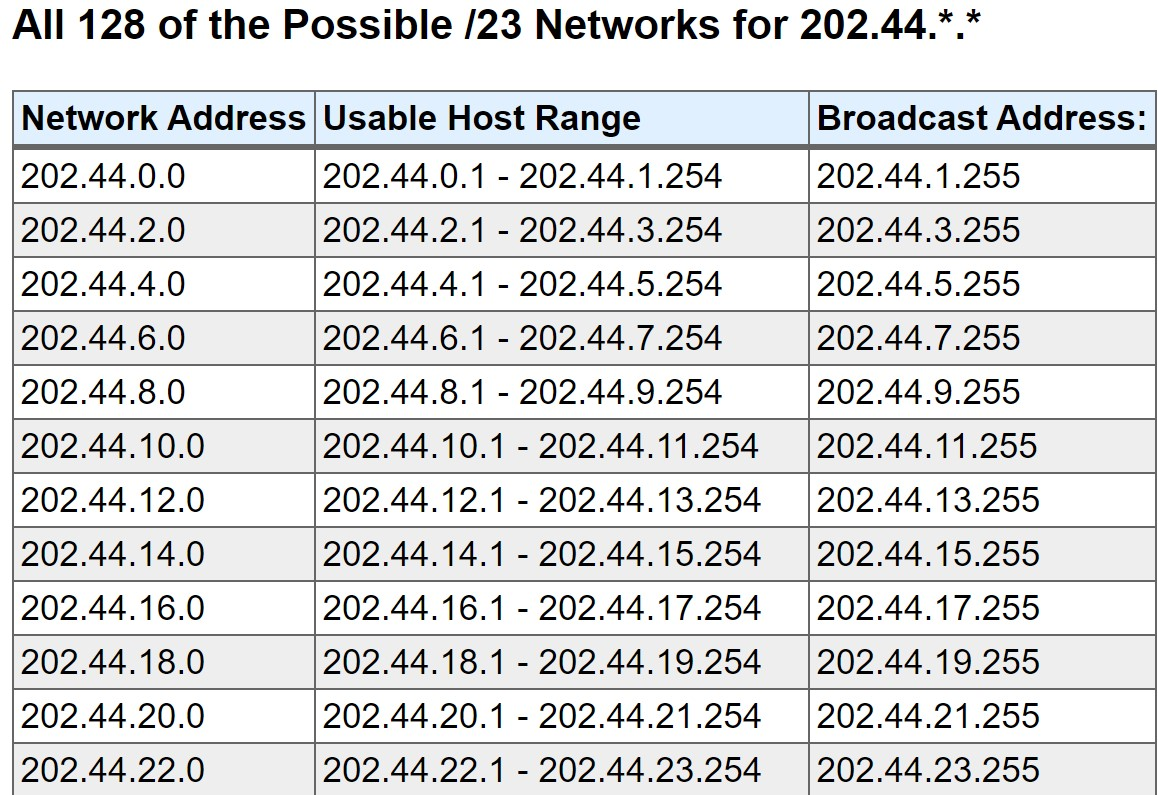
\includegraphics[scale=0.7,cframe=blue 0.5pt 3pt]{./FIG/C23.jpg}
              \caption{Possible subnets for /23 }
          \end{figure}


          With subnet mask (/23) PC1 and PC2 falls under one subnet similarly PC3 and PC4 falls under different subnet. So ping is possible between between PC1 and PC2 and similarly between PC3 and PC4 but ping failed between different subnet.

    \item \textbf{ Change the subnet mask to 255.255.252.0 and test the connectivity from one computer to
              another using ping.}

          \addtocontents{lol}{\protect\subsubsection*{C.4: Subnet mask : 255.255.252.0}}

          \CMD{./CODES/C4P1-4.txt}{Ping from PC1 to PC4}
          \CMD{./CODES/C4P2-1.txt}{Ping from PC2 to PC1}
          \CMD{./CODES/C4P3-2.txt}{Ping from PC3 to PC2}
          \CMD{./CODES/C4P4-3.txt}{Ping from PC4 to PC3}


          \begin{figure}[H]
              \centering
              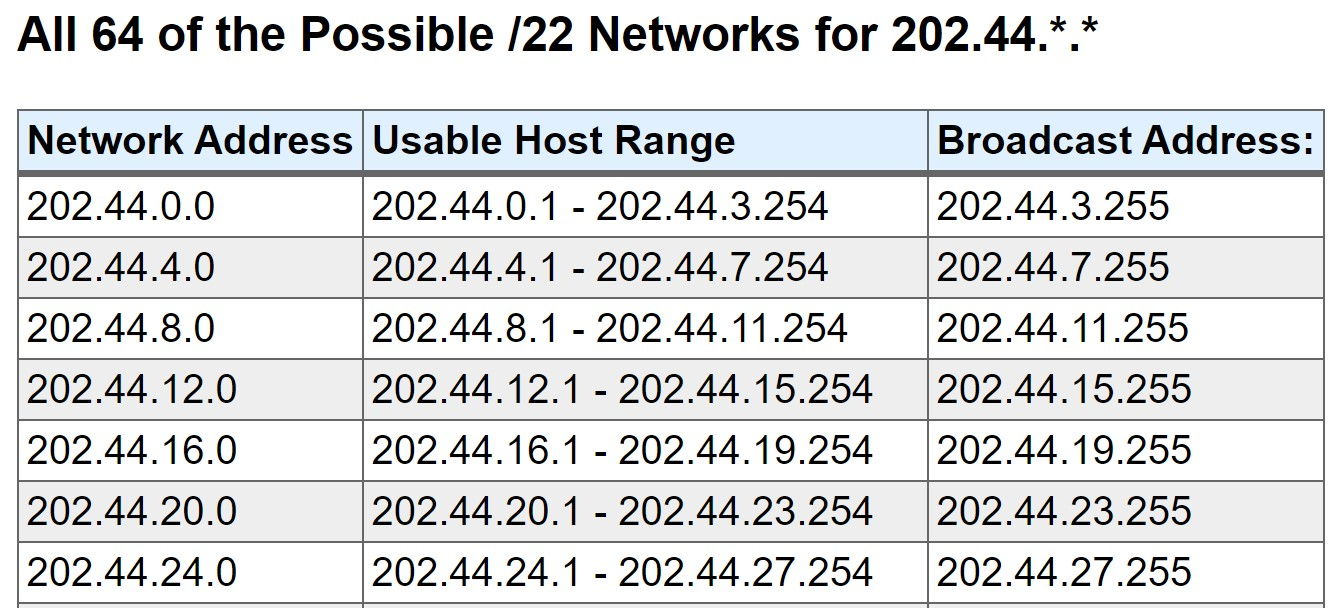
\includegraphics[scale=0.58,cframe=blue 0.5pt 3pt]{./FIG/C22.jpg}
              \caption{Possible subnets for /22 }
          \end{figure}


          With Subnet mask (/22) we can clearly see from above table that all PCs falls under same subnet hence Ping is possible between any two PCs.



    \item \textbf{ Change the subnet mask to 255.255.248.0 and test the connectivity from one computer to
              another using ping.}

          \addtocontents{lol}{\protect\subsubsection*{C.5: Subnet mask : 255.255.248.0}}

          \CMD{./CODES/C5P1-4.txt}{Ping from PC1 to PC4}
          \CMD{./CODES/C5P2-1.txt}{Ping from PC2 to PC1}
          \CMD{./CODES/C5P3-2.txt}{Ping from PC3 to PC2}
          \CMD{./CODES/C5P4-3.txt}{Ping from PC4 to PC3}

          \begin{figure}[H]
              \centering
              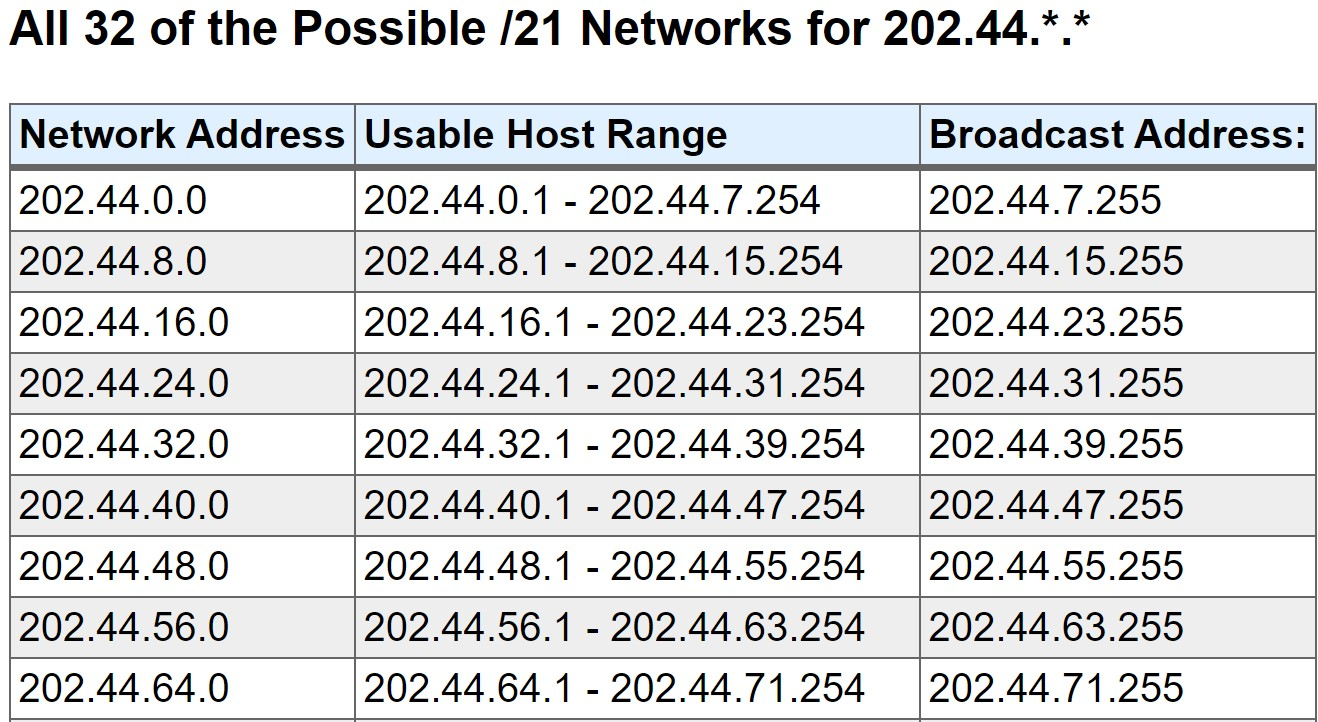
\includegraphics[scale=0.63,cframe=blue 0.5pt 3pt]{./FIG/C21.jpg}
              \caption{Possible subnets for /21 }
          \end{figure}

          With Subnet mask (/21) we can clearly see from above table that all PCs falls under same subnet hence Ping is possible between any two PCs.



\end{enumerate}




\pagebreak
%
%
%
%

%%%%%%%%%%%%%%%%%%%%%DDDDDDDDDDDDDDDDDDDDDDDD
%%%%%%%%%%%%%%%%%%%%%DDDDDDDDDDDDDDDDDDDDDDDD
%%%%%%%%%%%%%%%%%%%%%DDDDDDDDDDDDDDDDDDDDDDDD
%%%%%%%%%%%%%%%%%%%%%DDDDDDDDDDDDDDDDDDDDDDDD
%%%%%%%%%%%%%%%%%%%%%DDDDDDDDDDDDDDDDDDDDDDD
%
%
%
%
%

\addtocontents{lol}{\protect\subsection*{\HRule \\ Activities D\\ \HRule}}

\addtocontents{lof}{\protect\subsection*{\HRule \\ Activities D\\ \HRule}}

\subsubsection{Activities D}

{\bfseries \textit{D. You have given IP addresses of 202.20.20.0/24 from your ISP. You are assigned to divide this
        address range equally for five different departments A, B, C, D, E and two networks F and G for
        interconnection of routers, which are connected as shown in given figure 2 below. Allocate the
        IP address range for each of the departments with their network address, broadcast address and
        subnet mask. Also list out the unused range of IP addresses (if any). Also enable static routing
        in between each of the department’s network as well as to Internet via ISP Router.}}


\begin{figure}[H]
    \centering
    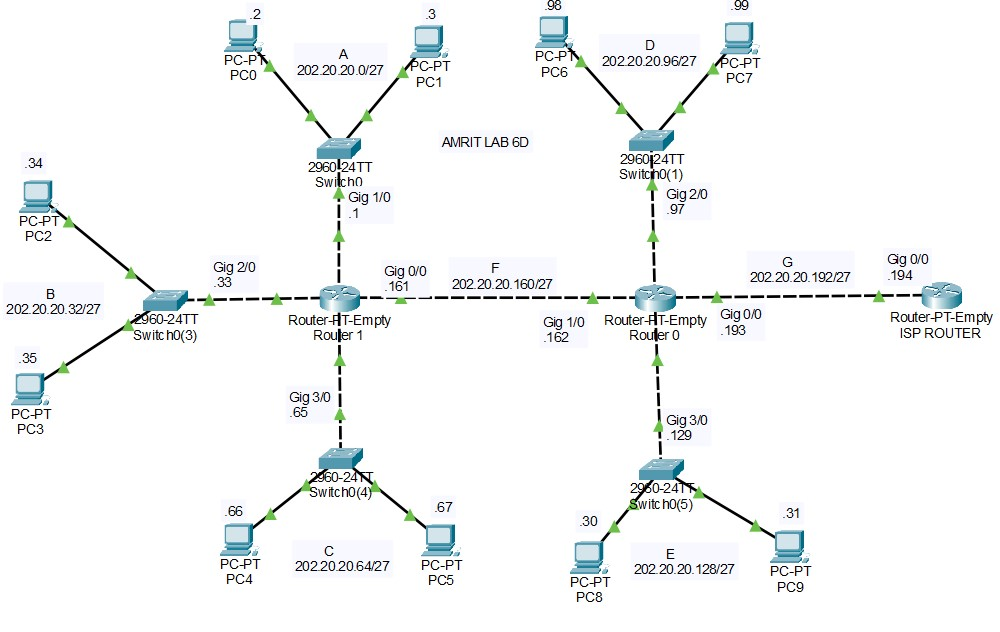
\includegraphics[scale=0.8,cframe=blue 0.5pt 3pt]{./FIG/Lab6D.jpg}
    \caption{Network topology Lab 6D}
\end{figure}

As we are asked to divide the given Ip range into 7 different network equally , I divide it into 30 usable host for each subnet with the help of subnet mask 255.255.255.224 . There is still  unused range of IP from 202.20.20.224 - 202.20.20.255 .

\begin{figure}[H]
    \centering
    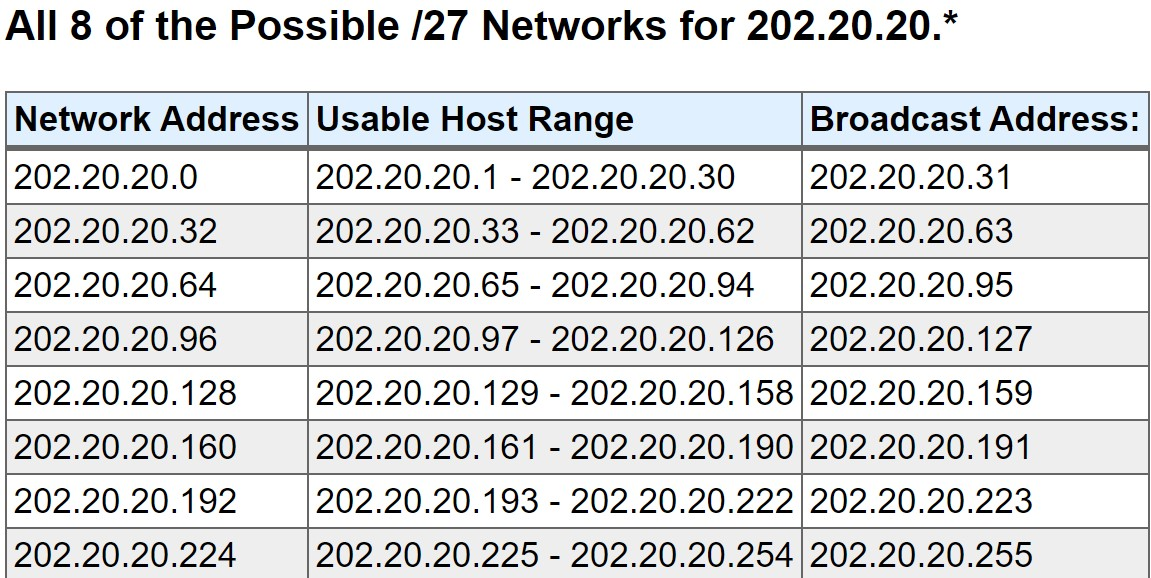
\includegraphics[scale=0.73,cframe=blue 0.5pt 3pt]{./FIG/D27.jpg}
    \caption{Possible subnets for /27 }
\end{figure}


I have used Default route and static route configuration for Static routing. In Router 1 all the outgoing traffic is forwarded to Router 0 (Gig 1/0) . For Router 0  Static route configuration is used for Network A, B and C , forwarded  Router 1(Gig 0/0) where as for Isp Router Default Route is used by forwarding all unknown destination to ( ISP ROUTER Gig 0/0) . Similarly for ISP Router default route config is used to forward all unknown to Router 0(Gig 0/0). To prove my point I have attached the Output of ping command  from different PCs of different Network.

\CMD{./CODES/DP1-4.txt}{Ping from PC1 to PC4}
\CMD{./CODES/DP4-7.txt}{Ping from PC4 to PC7}
\CMD{./CODES/DP2-ri.txt}{Ping from PC2 to ISP ROUTER}



\pagebreak

%%
%
%
%
%
%%%%%%%%%%%%%%%%%%EEEEEEEEEEEEEEEEEEEEEEEEEEE
%%%%%%%%%%%%%%%%%%EEEEEEEEEEEEEEEEEEEEEEEEEEE
%%%%%%%%%%%%%%%%%%EEEEEEEEEEEEEEEEEEEEEEEEEEE
%%%%%%%%%%%%%%%%%%EEEEEEEEEEEEEEEEEEEEEEEEEEE
%%%%%%%%%%%%%%%%%%EEEEEEEEEEEEEEEEEEEEEEEEEEE
%%
%
%
%
%


\addtocontents{lol}{\protect\subsection*{\HRule \\ Activities E\\ \HRule}}

\addtocontents{lof}{\protect\subsection*{\HRule \\ Activities E\\ \HRule}}

\subsubsection{Activities E}

{\bfseries \textit{E. You have given a IP addresses of 202.70.90.0/24. You have to divide this address range for
        different departments A, B, C, D and E interconnected as shown in figure 2 above, each
        department having 54, 27, 18, 12, 6 number of hosts. In addition to this there are two networks
        F and G having only two host in each. Allocate the IP address range for each of the sub-
        networks with their network address, broadcast address and subnet mask. Also list out the
        unused range of IP addresses (if any). Also enable static routing in between each of the
        department’s network as well as to Internet via ISP Router.}}




\begin{figure}[H]
    \centering
    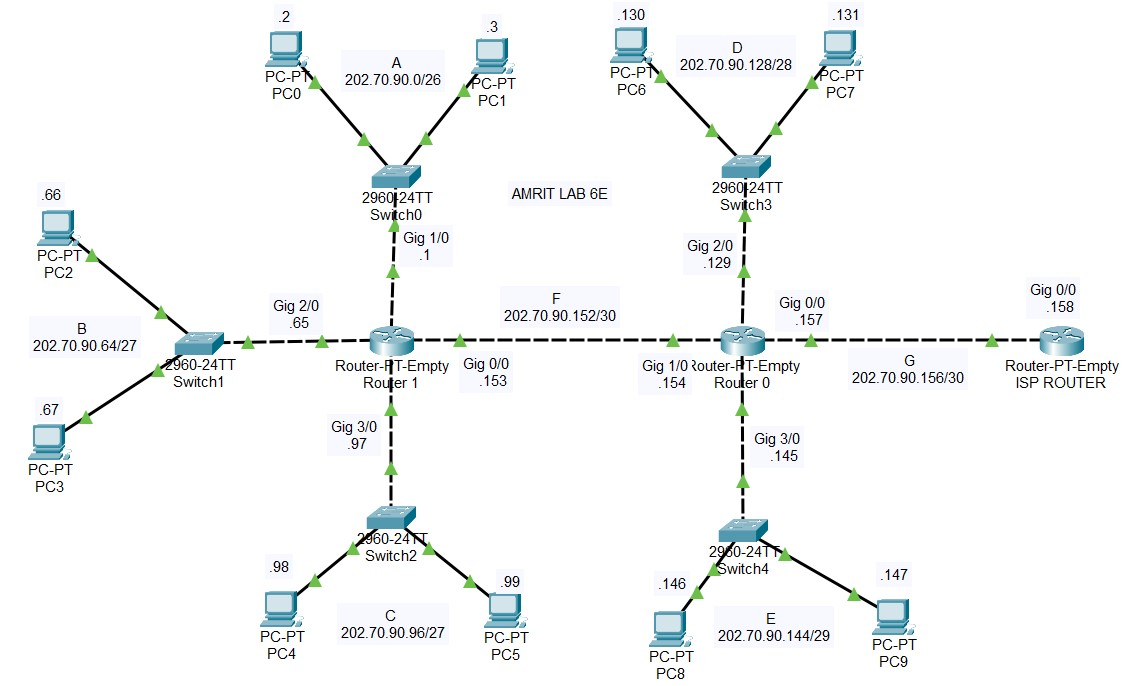
\includegraphics[scale=0.75,cframe=blue 0.5pt 3pt]{./FIG/Lab6E.jpg}
    \caption{Network topology Lab 6E}
\end{figure}

\begin{figure}[H]
    \centering
    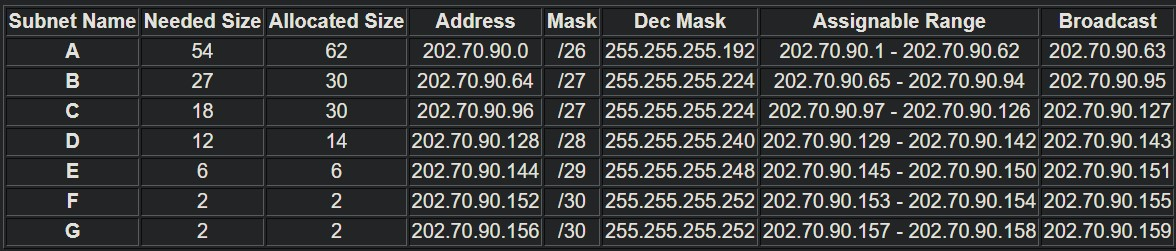
\includegraphics[scale=0.73,cframe=blue 0.5pt 3pt]{./FIG/EV.jpg}
    \caption{Possible subnets with VLSM}
\end{figure}

There is unused IP Range from 202.70.90.160 - 202.70.90.255 .\\

I have used Default route and static route configuration for Static routing. In Router 1 all the outgoing traffic is forwarded to Router 0 (Gig 1/0) . For Router 0  Static route configuration is used for Network A, B and C , forwarded  Router 1(Gig 0/0) where as for Isp Router Default Route is used by forwarding all unknown destination to ( ISP ROUTER Gig 0/0) . Similarly for ISP Router default route config is used to forward all unknown to Router 0(Gig 0/0). To prove my point I have attached the Output of ping command  from different PCs of different Network.

\CMD{./CODES/EP1-4.txt}{Ping from PC1 to PC4}
\CMD{./CODES/EP4-7.txt}{Ping from PC4 to PC7}
\CMD{./CODES/EP2-ri.txt}{Ping from PC2 to ISP ROUTER}


\pagebreak



%%%%%%%%%%%%%%%%%%%%%%%%%%%2222222222222222222222222222222222222222
\addtocontents{lof}{\protect\subsection*{\HRule \\ Question 2\\ \HRule}}

\begin{Q}
    {
        Explain subnetting and VLSM with their importance in networking with suitable examples.
    }
\end{Q}

\begin{A}
    {
        Subnetting is the technique to prevent formation of complex large network and instead divide that network and create fast, efficient and secure network and routes.
        There are two subnetting techniques  (VLSM) variable Length Subnet Mask and (FLSM) fixed length. In FLSM all subnet has equal host and uses same subnet mask wasting lot of IP whereas  VLSM  Subnet has variable host and uses different subnet mask with reduced ip wastage.

        Some importance of subnetting are:
        \begin{itemize}
            \item Divides the broadcast domain improving the network performance
            \item The data intended for host within the same subnet will not leave the subnet thus reducing the congestion and improving security.
            \item It also helps to organize the complex network into subnets based on departments and location.
        \end{itemize}




        In the example below IOE was given 202.70.90.0/24  ranges of IPs.Without subnetting the whole IOE network become complex and unsecure as  Student and Department are under same subnet (/24) but after the VLSM subnetting is done  as Student has need of 120 host and Department has need of 50 host only so they are divided into two subnets using subnet mask (/25) and (/26) respectively.  There is still unused IP range from 202.70.90.192 - 202.70.90.255 which wil be beneficial for further expansion of departments and future use.

        \begin{figure}[H]
            \centering
            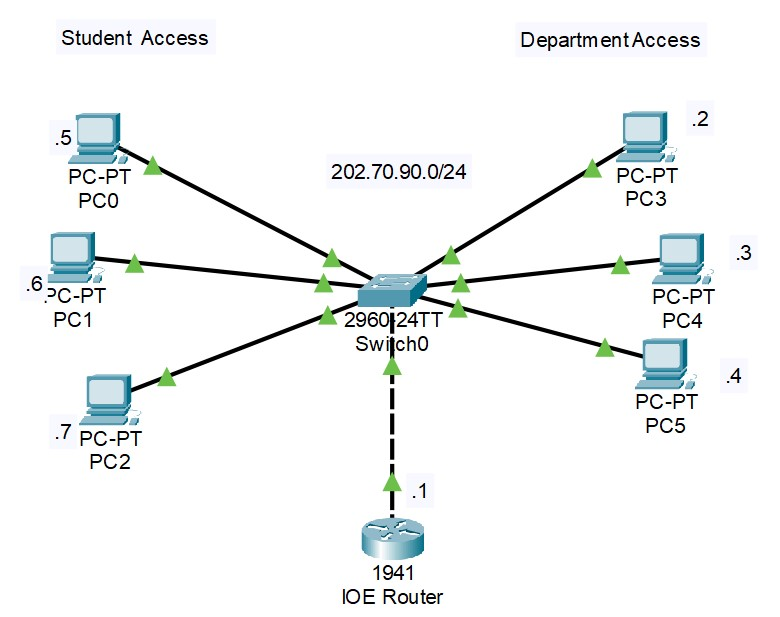
\includegraphics[scale=0.85,cframe=blue 0.5pt 3pt]{./FIG/IOEB.jpg}
            \caption{IOE network before subnetting}
        \end{figure}

        \begin{figure}[H]
            \centering
            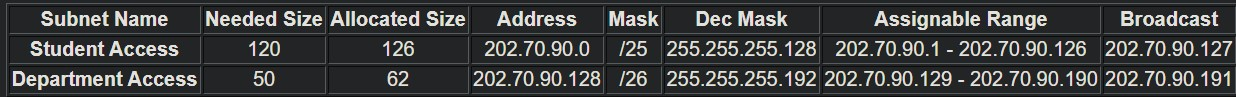
\includegraphics[scale=0.7,cframe=blue 0.5pt 3pt]{./FIG/SubTab.jpg}
            \caption{Details of IOE Subnets}
        \end{figure}


        \begin{figure}[H]
            \centering
            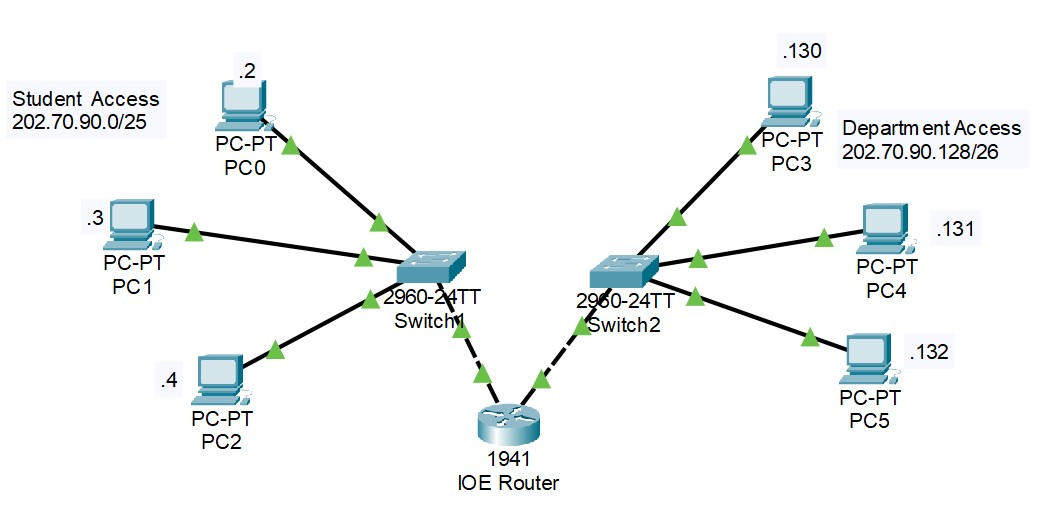
\includegraphics[scale=0.75,cframe=blue 0.5pt 3pt]{./FIG/IOEA.jpg}
            \caption{IOE network after subnetting}
        \end{figure}


    }
\end{A}

%%%%%%%%%%%%%%%%%%%%%%%%%%%%%%%%%%%33333333333333333333

\begin{Q}
    {
        What is classless routing? Why is it used in Internet system? Explain with suitable
        examples.
    }
\end{Q}

\begin{A}
    {
        In Classful Routing subnet mask are not sent with updates instead the default Subnet mask for particular class based on IP is used. But in Classless Routing Subnet mask are also sent along with IP. Classless Routing Supports VLSM (Variable Length Subnet Mask) is supported and also CIDR (Classless Inter-Domain Routing).\\

        As we know :
        \begin{itemize}
            \item Class B with a mask of 255.255.0.0 can support 65, 534 addresses
            \item Class C with a mask of 255.255.255.0 can support 254 addresses
        \end{itemize}

        But if there is need of 600  or 5000  host just Class C will be insufficient and Class B will waste large no of IPs. However if Classless routing is implemented with VLSM it will prevent ip wastage and network collision.

    }
\end{A}


%%%%%%%%%%%%%%%%%%%
\pagebreak

\section{Conclusion}


In this lab we familiarize ourselves with Subnetting , VLSM ,CIDR and Subnet mask. In Activity A we created the subnet with the help of subnet mask and try to communicate between different subnet as switch as medium but failed However, In Activity B when  central switch is replaced by Router Ping is successful. Similarly we explored the concept of subnet in Activity C even further . In Activity D we created 7 subnet of Equal host  and configured the static route between the router . Similarly in Activity E VLSM technique is used.

\end{document}